\chapter{Background and History\label{section:history}}
\section{Background}\label{section:background}

\subsection{Sensor technology}
At its core, sensors are just some photodiodes that can convert photons
into electrical charge. In this section we will cover two common sensor this is
done, as well as a brief list of pros and cons for each.

\subsubsection{Complementary Metal Oxide Semiconductor Sensors}
\textit{Complementary Metal Oxide Semiconductor} (CMOS) sensors are very old
sensors, being around since the 1960s. Over the years due to lithography
improvements they have become very good, being able to compete with with
\textit{Charged Couple Device} (CCD) sensors which are known for better image
quality technology. While CCDs have a better image quality, it requires much
more power than CMOS which can be up to 100 times less power hungry
\cite{CMOSReview}. This means that in many mobile devices and many other low
power devices wants CMOS over CCDs.

CMOS sensors are similar to the CMOS memory chips, unlike the memory chips the
sensors use photodiodes along with amplifiers \cref{fig:cmosvsccd} over
transistors. The amplifiers exist to well, amplify the signal. This design
allows us to access individual pixels quickly using random access on top of being
able to read out R, G and B signals simultaniously\cite{cmosAlen}. Because
there are so many photodiodes along with amplifiers, electrical fluctuation
is created. This causes intermittencies in the quality of the image, there are
a number of noise reduction algorithms that can be applied on the image to
remove these.

Curious readers can have a look at \cite{CMOSReview} \cite{ieeeCMOS} for a more
in depth overview of what CMOS sensors are.

\subsubsection{Charged Couple Device Sensors}
\textit{Charged Couple Device} (CCD) sensors were for a long time considered
significantly better than CMOS. It works using capacitors next to the
photodiodes to create voltage out of charge which is then read out in a serial
manner. Unlike CMOS, CDD allows you to design very small pixel sizes as the
pixels themselves do not require much real estate. The downside of this is that
this creates a lot of heat, requiring good cooling which is not always
available. In \cref{fig:cmosvsccd} we can see how the CCD sensor looks like on
a high level. Because CCD sensors read the signals row by row, if there are some
pixels are very bright it can create visual effects for the entire row.

\begin{figure}
    \begin{center}
        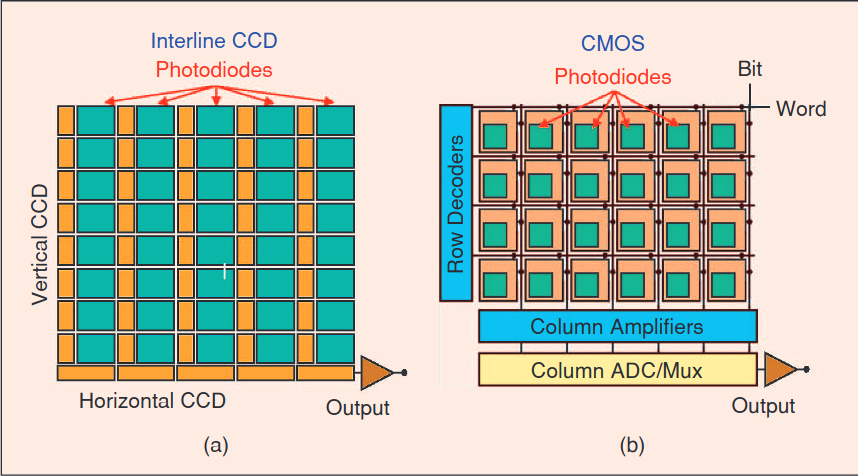
\includegraphics[width=0.55\textwidth]{figures/cmos_vs_cdd}
    \end{center}
    \caption{CMOS vs CDD comparison\cite{ieeeCMOS}}\label{fig:cmosvsccd}
\end{figure}


\newpage
\subsection{Image Signal Processors} \label{section:isp}
\textit{Image Signal Processors} (ISPs) are a highly secretive piece of
hardware. There are few systems that say they even have one, and even fewer
that explain how they work. To understand how ISPs work, we will be using the
Raspberry Pi\footnote{https://datasheets.raspberrypi.com/camera/raspberry-pi-camera-guide.pdf}
\footnote{https://datasheets.raspberrypi.com/camera/raspberry-pi-image-signal-processor-specification.pdf},
it is the only one that is open source (except for the RTL code) along with an
open specification. ISPs can differ slightly though the idea is roughly the
same across the board.

In this section we will give an overview of what ISPs typically do and how they
function.

So ISPs, what exactly are they? As the name suggests, they process image
signals. When an image come from the sensor the signal (image) contains a lot
of redundant and unprocessed information. The sensor is also also not quite
calibrated to the real world environment, a lot of things are simply wrong with
it. Correcting these is an expensive process, so much so that there is a HW
block in camera systems that does this for you.

The isp has a couple steps, most work something along the lines of

\begin{figure}[htpb]
    \centering
    \subfloat[Blue Channel]{
        
\includegraphics[width=0.2\textwidth]{figures/bayer_frame_blue.png}
        \label{fig:bayer_blue}
    }
    \qquad
    \subfloat[Green Channel]{
        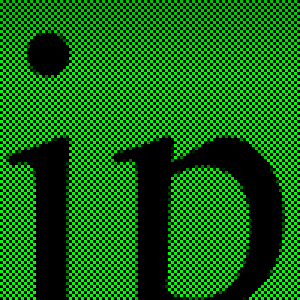
\includegraphics[width=0.2\textwidth]{figures/bayer_frame_green.png}
        \label{fig:bayer_green}
    }
    \qquad
    \subfloat[Red Channel]{
        
\includegraphics[width=0.2\textwidth]{figures/bayer_frame_red.png}
        \label{fig:bayer_red}
    }
    \qquad
    \subfloat[Full Bayer Frame]{
        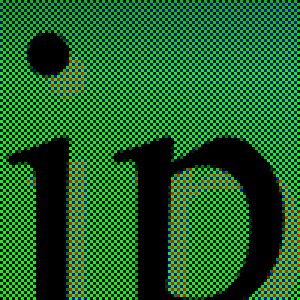
\includegraphics[width=0.2\textwidth]{figures/bayer_frame.png}
        \label{fig:bayer_full}
    }
    \qquad
    \subfloat[Final image]{
        
\includegraphics[width=0.2\textwidth]{figures/bayer_final}
        \label{fig:bayer_final}
    }
    \qquad
    \subfloat[Bayer pattern]{
        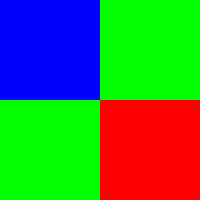
\includegraphics[width=0.2\textwidth]{figures/bayerpattern.png}
        \label{fig:bayer_pattern}
    }

    \caption[Bayer demosaicing]{Bayer demosaicing, \textit{source: https://en.wikipedia.org/wiki/Demosaicing}}
    \label{fig:bayer_channels}
\end{figure}

\begin{enumerate}
    \item Receive raw sensor data, often a Bayer image or similar

    \item Demosaic the image, i.e. extracting the pixel data from the raw
        image. The is often done using a Bayer like filter, many exist though
        they all work in the same way. In \cref{fig:bayer_channels} we can see
        how each of these channels are extracted. Once extracted they are
        combined into the final image as seen in \cref{fig:bayer_final}. One
        way this can be done is taking the average of each nearby pixel and
        interpolating them into a single one. This is quite crude compared to
        the real thing but the idea is the same. \cref{fig:bayer_pattern}

    \item The ISP then begins applying the autocontrol algorithms, the standard
        ones are known as the 3A algorithms for auto white balancing, gain, and
        exposure control. These will be covered in a bit more detail in
        \cref{section:autocontrol}.

    \item After processing the image in the ISP, the ISP then gives the image
        to the application that requested the image. The ISP also re-calibrates
        the autocontrol parameters based on the ones that were computed for the
        current frame. This is in order to correct for example white balancing,
        if coming from a very dark room into a very light room, it uses the
        current parameters to improve the white balancing.

\end{enumerate}

\subsubsection{Autocontrol algorithms} \label{section:autocontrol}

When people talk about their images being unedited, most do not realize that all
photos are edited to a degree. Some better than others, autocontrol algorithms
today can process an image quite heavily. This section will give an overview of
what autocontrol algorithms are, though not the inner workings of these
algorithms.

Effectively all ISPs today implement at the very least the 3A (\textit{Auto
White Balancing} (AWB), and \textit{Auto Gain Control} (AGC), \textit{Auto
Focus Control} (AFC)) algorithms. When the ISP receives metadata from the
sensor, it uses the AFC algorithm to focus on a specific object that the user
tries to focus on. Similarly, the AGC algorithm is used to make sure that the
image wll not be too bright or dark. AWBs purpose on the other hand is to make
sure that the temperature of the image is correct. Blue being cold and yellow
being warm, it balances the whites to reflect reality as closely as possible.

On top of the 3A algorithms, there are a lot more that the ISP often does. For
example there is often some lens shading, color correction and more. In
\cref{fig:lens_shading} we can see an example of how the ISP has fixed the image.
In \cref{fig:with_shading} the corners are significantly darker than the center.
While in \cref{fig:without_shading} the whole image is equally lit.

\begin{figure}[htpb]
    \centering
    \subfloat[With lens shading]{
        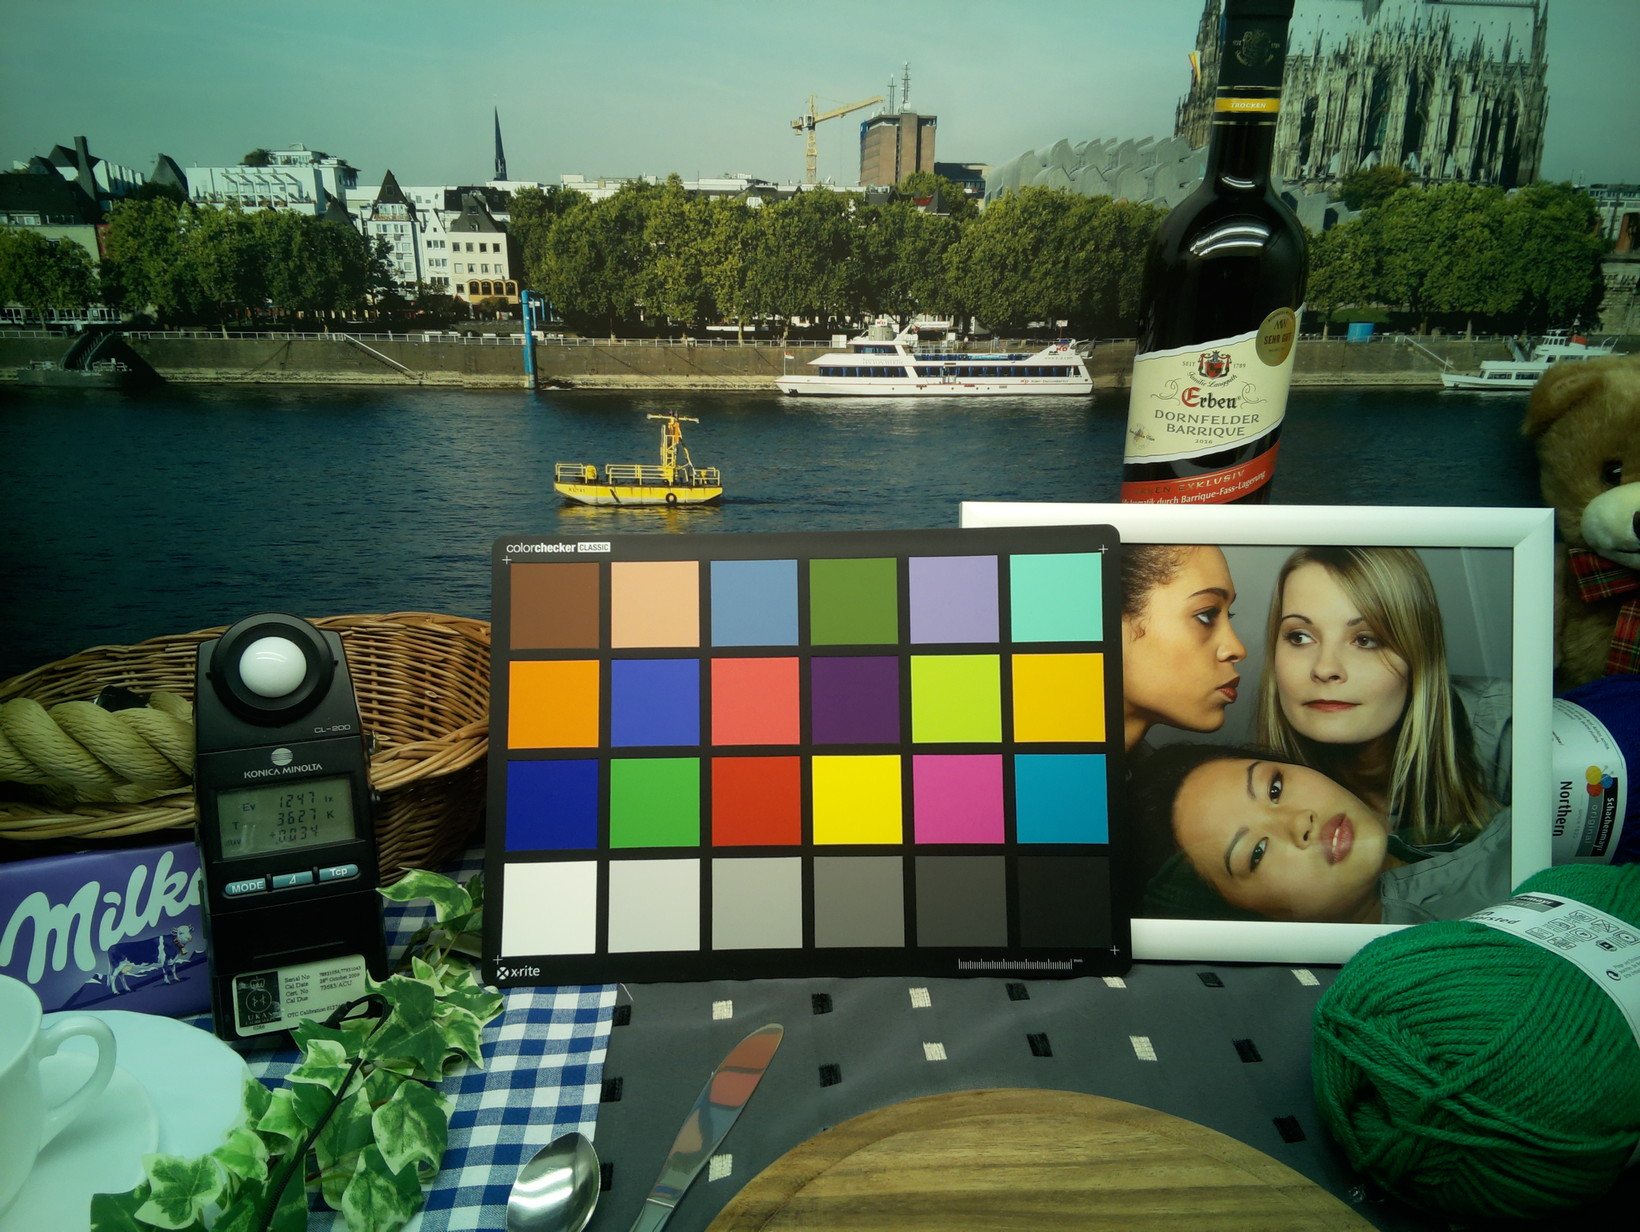
\includegraphics[width=0.4\textwidth]{figures/alsc-none.jpg}
        \label{fig:with_shading}
    }
    \qquad
    \subfloat[Without lens shading]{
        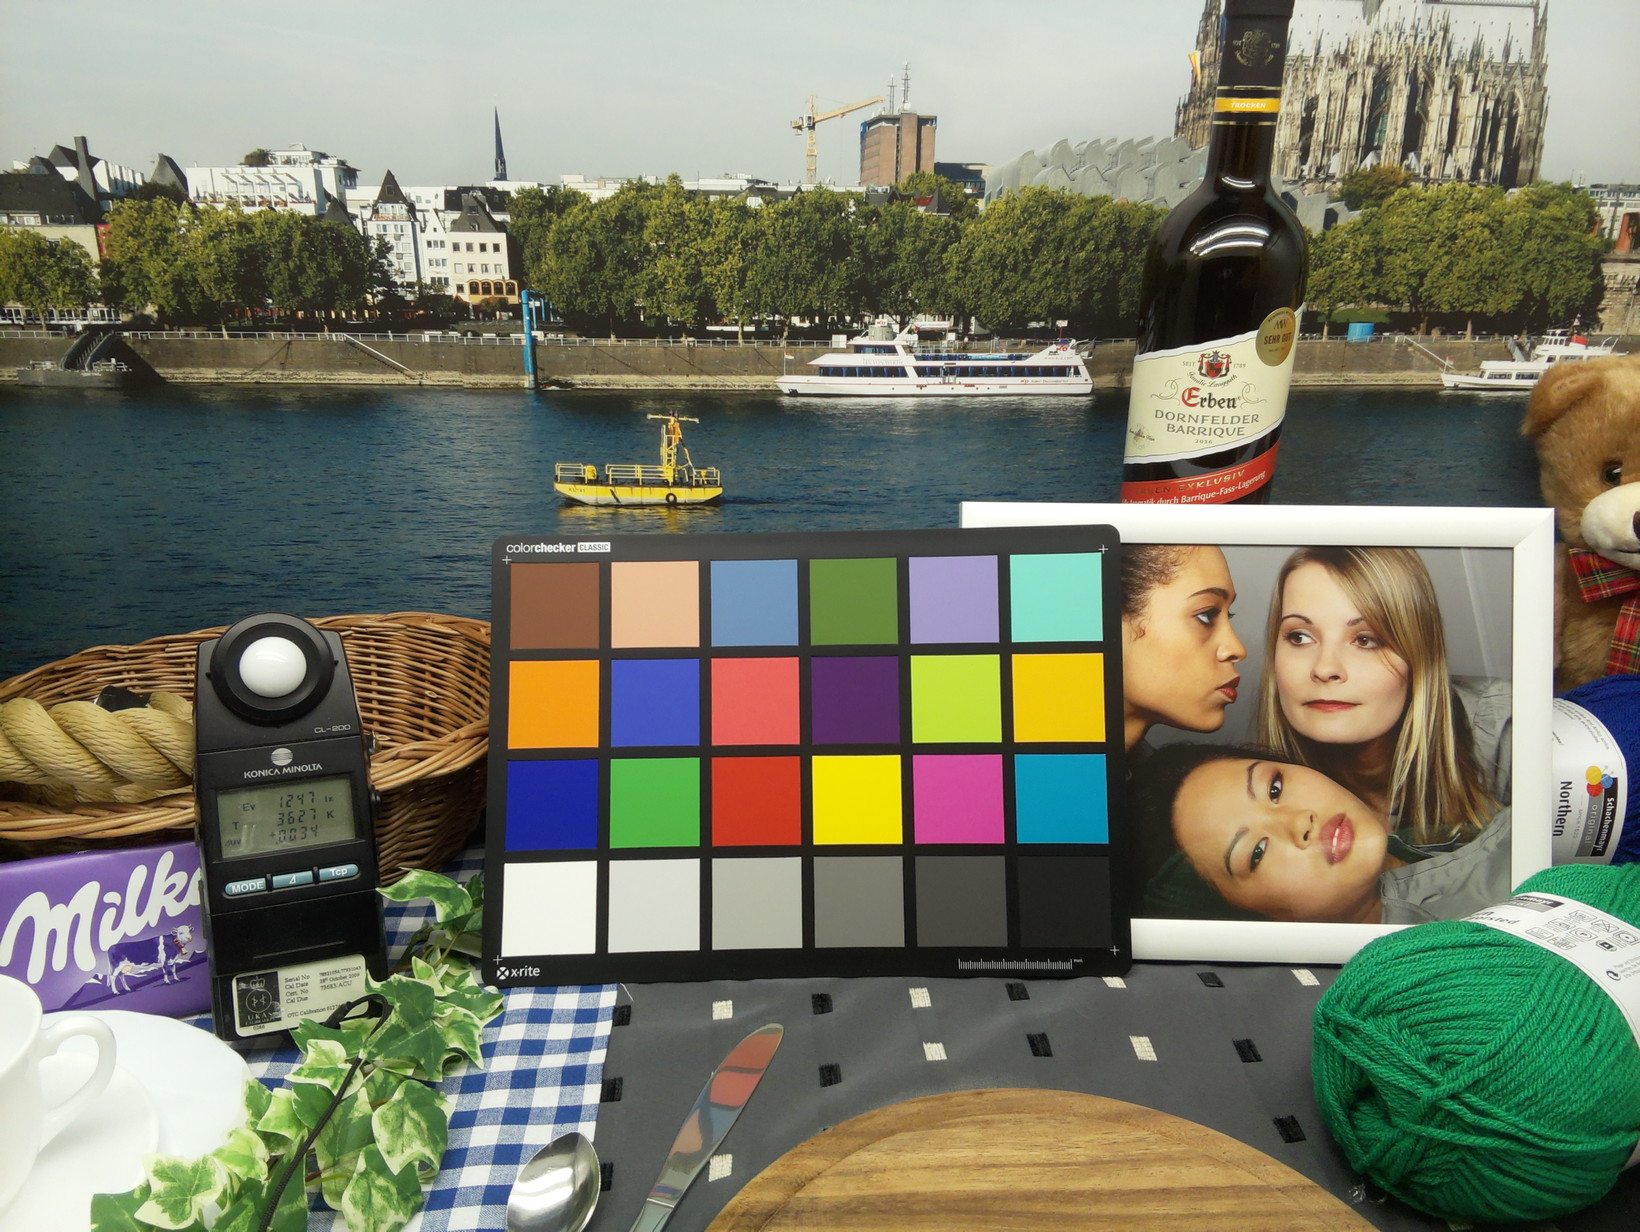
\includegraphics[width=0.4\textwidth]{figures/alsc-both.jpg}
        \label{fig:without_shading}
    }

    \caption{Different lens shading corrections. \textit{Photo by Naush Patuk used with permission}}\label{fig:lens_shading}
\end{figure}

\subsubsection{Image Processing and Tiles}
The Raspberry Pi ISP is divided into two sections, the front- and back end.
Though the front end has some image processing capabilties, being able to scale
and crop images. Its main responsibility is to write images to main memory,
providing an
AXI\footnote{https://developer.arm.com/documentation/ihi0051/latest} interface
to give the ISP frames. While doing this, it provides the backend with some
statistics of the image. These statistics consist of for example histograms
of color counts etc.

The backend then reads these images that the frontend has provided. Unlike how
applications deal with full frames, the backend deals with \textit{tiles}. The
Raspberry Pi uses tiles that are 640x640 aligned to 64 bits. This is done in
order to reduce the amount of memory required to process an image and speed up
memory access. By limiting it to tiles of the image, significantly less memory
is required for a 4K image to be processed. Additionally this means that the
image processing can be paralellized, by splitting the image into several
chunks the ISP can safely process the image in paralell.

\subsection{Transport layer}
In this section we will cover different common technologies that have been used
to transport images along with an insight into when they are used.

\subsubsection{CSI-2}
CSI-2 is a technology to transport sensor data over short distances very
quickly. While being initially made for mobile, the technology has moved to
automotive. Because of this, CSI-2 has been made to transport data over a few
centimeters. This has made it slightly more difficult in the automotive
industry, as cars are larger than a few centimeters. The solution for this is
often to have another technology for the longer part, once it is within range
converting it back to CSI-2.

CSI-2 uses two different technologies, namely C-PHY and D-PHY. These can
transport data at different speeds. Along with the fast C-PHY/D-PHY lanes,
control lanes are also provided that control the camera over I$^2$C.

D-PHY uses a dedicated lane for clock, this means that it only has two lanes for
data transport. It is a very simple synchronous protocol, it does not encode
bits in any way.

Unlike D-PHY, C-PHY does not have a dedicated lane for clock. It uses all lanes
for both clock and data transport, embedding the clock implicitly into the
data. C-PHY encodes the bits into symbols, the encoder then guarantees that
there will be at least one edge in the signal. This allows the receiver to
derive a clock. Encoding the data, allows one to pass more information to the
receiver at once opposed to if no encoding would be done.

TODO add images?

\subsubsection{USB}

\section{History}
In this section we will cover the history of cameras on Linux.

In the early days cameras were quite simple, there effectively was just the
"press button" followed by receiving a picture. This process did not allow for
much customization. This was the case with most cameras such as webcams where
the camera sensors were "smart sensors". This meant that the cameras had a small
ISP integrated into them, they could do the processing internally. Even the
integrated laptop ones were just USB devices that spit out images. Linux had
initially had lacking support for this, but in the early 2000s Video For Linux
(V4L, later V4L2 for version 2) was developed. This covered most of the use
cases at the time. V4L grew organically over the years, it developed the
features that were needed as they were needed. This meant that there was no
large plan being executed, in turn the design that grew became a bad one
\footnote{Direct documentation on what was wrong with the API has not really
been written, this is based on a discussion with Laurent Pitchard}.
In 1998 Bill Dericks began the design and development of V4L2 which we have in
use today.

\begin{wrapfigure}{r}{0.5\textwidth}
    \centering
    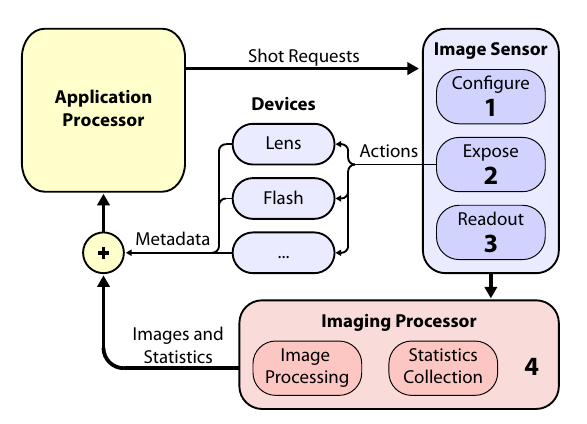
\includegraphics[width=0.48\textwidth]{figures/fcam_arch.png}
    \caption{FCam archictecture \cite{adams2010frankencamera}}
    \label{fig:fcam_api}
\end{wrapfigure}

In 2009 the Nokia N900 was released, this was a Linux based phone that was not
like most cameras at the time. It provided interfaces for customizing just
about everything. From ISPs to Image Processing Algorithms (IPAs), this meant
that the current way camera APIs worked was no longer maintainable. It
required that the application would manage everything, computing the
histograms, configuring the autocontrol etc.. While this was doable for a
company on the scale of Nokia at the time, it was not for anyone else. Enter
Frankencamera\cite{adams2010frankencamera}; this was an effort at the time
to create an API that allowed the user to express the different options that
cameras needed. This effort was lead by Stanford and Nokia, it is what most
modern APIs are based on at a high level. It was built on top of V4L2,
providing a more user friendly API than the kernel drivers themselves.

Like its successors covored in \cref{section:currentAPIs}, the Frankencam API
was a request based API. The idea with it was to allow for the user to control
the cameras very well. \cref{fig:fcam_api} shows the block diagram of how the
API worked. The application would request a capture, the sensor gets
reconfigured based on the request. After which it would capture the image with
which ever peripherals the user has and finally forward the image to the ISP.
The ISP then processes the image and gives it to the application along with the
metadata. This will look very similar to how modern APIs work which is covered
in \cref{section:currentAPIs}.

Before Frankencam many camera APIs were stateful\cite{experimentalCompPhot},
they only had one state that controlled the sensor. This meant that when you
wanted to capture multiple images with multiple settings the changes would take
effect at an unpredictable time in the future. While also adding latency to
manage the state internally, it also meant that you had to clear the capture
pipeline so that you could guarantee that the settings were correct. This was a
very complex process, though state was important; it was placed in the wrong
place. This lead to the creation of the request based API, where the
application would manage the state and the camera would simply accept requests.

